% answers.tex —— 1998 年·全国卷·理科 · 参考答案与详细解析片段
% 由 tools/generate_projects.py 依来源总账自 1998/1998_数学真题_全国理_试题.md + 1998/1998_数学真题_全国理_解析正文.md + 1998/1998_数学真题_全国理_答案要点.md 生成，勿手改（改源 MD 后重跑）


\begin{gktip}
固定源 PDF 只有一页题面，没有答案和解析页。以下各题均依据题面独立复算；第 2、10、21、22、23 题的图形在 LaTeX 工程中以 TikZ/PGFPlots 矢量源重绘。
\end{gktip}

\begin{answer}
\gksolhead{1}{}

\textbf{题目}：

$\sin600^\circ$ 的值是\mbox{（　　）}

（A）$\dfrac12$　　（B）$-\dfrac12$　　（C）$\dfrac{\sqrt3}{2}$　　（D）$-\dfrac{\sqrt3}{2}$

\Needspace{4\baselineskip}
\textbf{解析}

\nopagebreak[4]
\[
600^\circ=360^\circ+240^\circ,
\]

\Needspace{5\baselineskip}
所以

\nopagebreak[4]
\[
\sin600^\circ=\sin240^\circ=-\frac{\sqrt3}{2}.
\]

因此选 D。

\gkanswer{答案：D}

\end{answer}
\begin{answer}
\gksolhead{2}{}

\textbf{题目}：

函数 $y=a^{|x|}\ (a>1)$ 的图象是\mbox{（　　）}
\nopagebreak[4]
\begin{center}% 1998 年全国卷理科第 2 题：函数 y=a^{|x|}（a>1）的四个图象选项
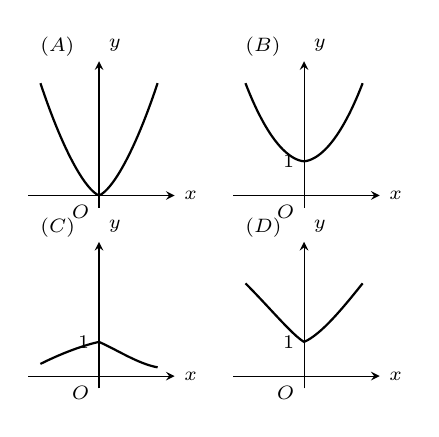
\begin{tikzpicture}[>=stealth, scale=0.62]
  \begin{scope}
    \node[font=\scriptsize, anchor=west] at (-1.4,3.05) {$(A)$};
    \draw[->] (-1.45,0)--(1.55,0) node[right, font=\scriptsize] {$x$};
    \draw[->] (0,-0.25)--(0,2.75) node[above right, font=\scriptsize] {$y$};
    \draw[thick] (-1.2,2.3) .. controls (-0.7,0.8) and (-0.25,0.1) .. (0,0)
      .. controls (0.25,0.1) and (0.7,0.8) .. (1.2,2.3);
    \node[below left, font=\scriptsize] at (0,0) {$O$};
  \end{scope}

  \begin{scope}[xshift=4.2cm]
    \node[font=\scriptsize, anchor=west] at (-1.4,3.05) {$(B)$};
    \draw[->] (-1.45,0)--(1.55,0) node[right, font=\scriptsize] {$x$};
    \draw[->] (0,-0.25)--(0,2.75) node[above right, font=\scriptsize] {$y$};
    \draw[thick] (-1.2,2.3) .. controls (-0.7,1.0) and (-0.25,0.72) .. (0,0.7)
      .. controls (0.25,0.72) and (0.7,1.0) .. (1.2,2.3);
    \node[below left, font=\scriptsize] at (0,0) {$O$};
    \node[left, font=\scriptsize] at (0,0.7) {$1$};
  \end{scope}

  \begin{scope}[yshift=-3.7cm]
    \node[font=\scriptsize, anchor=west] at (-1.4,3.05) {$(C)$};
    \draw[->] (-1.45,0)--(1.55,0) node[right, font=\scriptsize] {$x$};
    \draw[->] (0,-0.25)--(0,2.75) node[above right, font=\scriptsize] {$y$};
    \draw[thick] (-1.2,0.25) .. controls (-0.7,0.5) and (-0.25,0.65) .. (0,0.7)
      .. controls (0.35,0.55) and (0.8,0.25) .. (1.2,0.18);
    \node[below left, font=\scriptsize] at (0,0) {$O$};
    \node[left, font=\scriptsize] at (0,0.7) {$1$};
  \end{scope}

  \begin{scope}[xshift=4.2cm,yshift=-3.7cm]
    \node[font=\scriptsize, anchor=west] at (-1.4,3.05) {$(D)$};
    \draw[->] (-1.45,0)--(1.55,0) node[right, font=\scriptsize] {$x$};
    \draw[->] (0,-0.25)--(0,2.75) node[above right, font=\scriptsize] {$y$};
    \draw[thick] (-1.2,1.9) .. controls (-0.7,1.4) and (-0.25,0.85) .. (0,0.7)
      .. controls (0.35,0.85) and (0.8,1.4) .. (1.2,1.9);
    \node[below left, font=\scriptsize] at (0,0) {$O$};
    \node[left, font=\scriptsize] at (0,0.7) {$1$};
  \end{scope}
\end{tikzpicture}
\end{center}
\nopagebreak[4]
\Needspace{4\baselineskip}
\textbf{解析}

由于 $a>1$，当 $x$ 增大时，$|x|$ 先减小后增大。函数 $y=a^{|x|}$ 是偶函数，在 $x=0$ 处取得最小值 $1$，并且向左右两侧都递增。因此图象应关于 $y$ 轴对称，在原点上方经过 $(0,1)$，且两端向上增长。四个图象中只有 B 符合，选 B。

\gkanswer{答案：B}

\end{answer}
\begin{answer}
\gksolhead{3}{}

\textbf{题目}：

曲线的极坐标方程 $\rho=4\sin\theta$ 化成直角坐标方程为\mbox{（　　）}

（A）$x^2+(y+2)^2=4$　　（B）$x^2+(y-2)^2=4$

（C）$(x-2)^2+y^2=4$　　（D）$(x+2)^2+y^2=4$

\Needspace{4\baselineskip}
\textbf{解析}

\Needspace{5\baselineskip}
由极坐标关系

\nopagebreak[4]
\[
x=\rho\cos\theta,\qquad y=\rho\sin\theta,
\]

\Needspace{5\baselineskip}
原方程给出

\nopagebreak[4]
\[
\rho^2=4\rho\sin\theta=4y.
\]

\Needspace{5\baselineskip}
即

\nopagebreak[4]
\[
x^2+y^2=4y
\iff x^2+(y-2)^2=4.
\]

所以选 B。

\gkanswer{答案：B}

\end{answer}
\begin{answer}
\gksolhead{4}{}

\textbf{题目}：

两条直线 $A_1x+B_1y+C_1=0$，$A_2x+B_2y+C_2=0$ 垂直的充要条件是\mbox{（　　）}

（A）$A_1A_2+B_1B_2=0$　　（B）$A_1A_2-B_1B_2=0$

（C）$\dfrac{A_1A_2}{B_1B_2}=-1$　　（D）$\dfrac{B_1B_2}{A_1A_2}=1$

\Needspace{4\baselineskip}
\textbf{解析}

\Needspace{5\baselineskip}
两条直线的法向量分别为 $(A_1,B_1)$ 和 $(A_2,B_2)$。两直线垂直，当且仅当它们的方向向量垂直，等价于法向量也垂直，因此

\nopagebreak[4]
\[
A_1A_2+B_1B_2=0.
\]

选 A。

\gkanswer{答案：A}

\end{answer}
\begin{answer}
\gksolhead{5}{}

\textbf{题目}：

函数 $f(x)=\dfrac1x\ (x\neq0)$ 的反函数 $f^{-1}(x)=$\mbox{（　　）}

（A）$x\ (x\neq0)$　　（B）$\dfrac1x\ (x\neq0)$

（C）$-x\ (x\neq0)$　　（D）$-\dfrac1x\ (x\neq0)$

\Needspace{4\baselineskip}
\textbf{解析}

设 $y=1/x$，交换 $x,y$ 后仍得到 $y=1/x$，且定义域仍为 $x\neq0$。因此函数图象关于直线 $y=x$ 对称，反函数就是自身，选 B。

\gkanswer{答案：B}

\end{answer}
\begin{answer}
\gksolhead{6}{}

\textbf{题目}：

已知点 $P(\sin\alpha-\cos\alpha,\tan\alpha)$ 在第一象限，则在 $[0,2\pi]$ 内 $\alpha$ 的取值范围是\mbox{（　　）}

（A）$\left(\dfrac\pi2,\dfrac{3\pi}4\right)\cup\left(\pi,\dfrac{5\pi}4\right)$

（B）$\left(\dfrac\pi4,\dfrac\pi2\right)\cup\left(\pi,\dfrac{5\pi}4\right)$

（C）$\left(\dfrac\pi2,\dfrac{3\pi}4\right)\cup\left(\dfrac{5\pi}4,\dfrac{3\pi}2\right)$

（D）$\left(\dfrac\pi4,\dfrac\pi2\right)\cup\left(\dfrac{3\pi}4,\pi\right)$

\Needspace{4\baselineskip}
\textbf{解析}

\Needspace{5\baselineskip}
点在第一象限等价于

\nopagebreak[4]
\[
\sin\alpha-\cos\alpha>0,\qquad \tan\alpha>0.
\]

\Needspace{5\baselineskip}
第一式给出

\nopagebreak[4]
\[
\sin\alpha>\cos\alpha
\iff \alpha\in\left(\frac\pi4,\frac{5\pi}4\right)
\quad\text{（\text{在} }[0,2\pi]\text{ \text{内}）}.
\]

\Needspace{5\baselineskip}
第二式给出

\nopagebreak[4]
\[
\alpha\in\left(0,\frac\pi2\right)\cup\left(\pi,\frac{3\pi}2\right).
\]

\Needspace{5\baselineskip}
两者相交为

\nopagebreak[4]
\[
\alpha\in\left(\frac\pi4,\frac\pi2\right)
\cup\left(\pi,\frac{5\pi}4\right).
\]

所以选 B。

\gkanswer{答案：B}

\end{answer}
\begin{answer}
\gksolhead{7}{}

\textbf{题目}：

已知圆锥的全面积是底面积的 3 倍，那么该圆锥的侧面展开图扇形的圆心角为\mbox{（　　）}

（A）$120^\circ$　　（B）$150^\circ$　　（C）$180^\circ$　　（D）$240^\circ$

\Needspace{4\baselineskip}
\textbf{解析}

\Needspace{5\baselineskip}
设圆锥底面半径为 $r$，母线长为 $l$。全面积是底面积的 $3$ 倍，所以侧面积是底面积的 $2$ 倍：

\nopagebreak[4]
\[
\pi rl=2\pi r^2,
\qquad l=2r.
\]

\Needspace{5\baselineskip}
侧面展开扇形的弧长为 $2\pi r$，半径为 $l$，故其圆心角为

\nopagebreak[4]
\[
\theta=\frac{2\pi r}{l}=\pi=180^\circ.
\]

选 C。

\gkanswer{答案：C}

\end{answer}
\begin{answer}
\gksolhead{8}{}

\textbf{题目}：

复数 $-\mathrm{i}$ 的一个立方根是 $\mathrm{i}$，它的另外两个立方根是\mbox{（　　）}

（A）$\dfrac{\sqrt3}{2}\pm\dfrac12\mathrm{i}$　　（B）$-\dfrac{\sqrt3}{2}\pm\dfrac12\mathrm{i}$

（C）$\pm\dfrac{\sqrt3}{2}+\dfrac12\mathrm{i}$　　（D）$\pm\dfrac{\sqrt3}{2}-\dfrac12\mathrm{i}$

\Needspace{4\baselineskip}
\textbf{解析}

\Needspace{5\baselineskip}
已知 $i^3=-i$。另外两个立方根的辐角分别为

\nopagebreak[4]
\[
\frac{3\pi/2+2\pi}{3}=\frac{7\pi}6,
\qquad
\frac{3\pi/2+4\pi}{3}=\frac{11\pi}6.
\]

\Needspace{5\baselineskip}
所以它们为

\nopagebreak[4]
\[
\cos\frac{7\pi}6+i\sin\frac{7\pi}6
=-\frac{\sqrt3}{2}-\frac12i,
\]

\Needspace{5\baselineskip}
以及

\nopagebreak[4]
\[
\cos\frac{11\pi}6+i\sin\frac{11\pi}6
=\frac{\sqrt3}{2}-\frac12i.
\]

选 D。

\gkanswer{答案：D}

\end{answer}
\begin{answer}
\gksolhead{9}{}

\textbf{题目}：

如果棱台的两底面积分别是 $S,S'$，中截面的面积是 $S_0$，那么\mbox{（　　）}

（A）$2\sqrt{S_0}=\sqrt S+\sqrt{S'}$　　（B）$S_0=\sqrt{SS'}$

（C）$2S_0=S+S'$　　（D）$S_0^2=2SS'$

\Needspace{4\baselineskip}
\textbf{解析}

\Needspace{5\baselineskip}
棱台的截面边长沿高方向线性变化，所以中截面各对应边长是两底对应边长的平均值。面积开方与线性尺寸成正比，因而

\nopagebreak[4]
\[
\sqrt{S_0}=\frac{\sqrt S+\sqrt{S'}}2,
\]

\Needspace{5\baselineskip}
即

\nopagebreak[4]
\[
2\sqrt{S_0}=\sqrt S+\sqrt{S'}.
\]

选 A。

\gkanswer{答案：A}

\end{answer}
\begin{answer}
\gksolhead{10}{}

\textbf{题目}：

向高为 $H$ 的水瓶中注水，注满为止，如果注水量 $V$ 与水深 $h$ 的函数关系的图象如下图所示，那么水瓶的形状是\mbox{（　　）}
\nopagebreak[4]
\begin{center}% 1998 年全国卷理科第 10 题：V-h 图象与四个水瓶形状选项
\begin{tikzpicture}[>=stealth, scale=0.72]
  \begin{scope}[xshift=4.9cm]
    \draw[->] (0,0)--(0,2.5) node[above] {$V$};
    \draw[->] (-0.2,0)--(2.6,0) node[right] {$h$};
    \draw[thick] (0,0) .. controls (0.35,1.5) and (1.35,2.15) .. (2.0,2.2);
    \draw[dashed] (2.0,0)--(2.0,2.2);
    \node[below] at (2.0,0) {$H$};
    \node[below left] at (0,0) {$O$};
  \end{scope}

  \begin{scope}[xshift=-6.0cm,yshift=-3.4cm]
    \node at (0,2.55) {$(A)$};
    \draw (0,0) ellipse (0.34 and 0.09);
    \draw (0,2) ellipse (0.72 and 0.16);
    \draw (-0.34,0) -- (-0.72,2) (0.34,0) -- (0.72,2);
    \draw[dashed] (-0.34,0) arc (180:0:0.34 and 0.09);
    \draw (-0.34,0) arc (180:360:0.34 and 0.09);
  \end{scope}

  \begin{scope}[xshift=-2.3cm,yshift=-3.4cm]
    \node at (0,2.55) {$(B)$};
    \draw (0,0) ellipse (0.72 and 0.16);
    \draw (0,2) ellipse (0.34 and 0.09);
    \draw (-0.72,0) -- (-0.34,2) (0.72,0) -- (0.34,2);
    \draw[dashed] (-0.72,0) arc (180:0:0.72 and 0.16);
    \draw (-0.72,0) arc (180:360:0.72 and 0.16);
  \end{scope}

  \begin{scope}[xshift=1.4cm,yshift=-3.4cm]
    \node at (0,2.55) {$(C)$};
    \draw (0,0) ellipse (0.72 and 0.16);
    \draw (0,2) ellipse (0.72 and 0.16);
    \draw (-0.72,0) .. controls (-0.30,0.7) and (-0.30,1.3) .. (-0.72,2);
    \draw (0.72,0) .. controls (0.30,0.7) and (0.30,1.3) .. (0.72,2);
    \draw[dashed] (-0.72,0) arc (180:0:0.72 and 0.16);
    \draw (-0.72,0) arc (180:360:0.72 and 0.16);
  \end{scope}

  \begin{scope}[xshift=5.1cm,yshift=-3.4cm]
    \node at (0,2.55) {$(D)$};
    \draw (0,0) ellipse (0.52 and 0.13);
    \draw (0,2) ellipse (0.52 and 0.13);
    \draw (-0.52,0) -- (-0.52,2) (0.52,0) -- (0.52,2);
    \draw[dashed] (-0.52,0) arc (180:0:0.52 and 0.13);
    \draw (-0.52,0) arc (180:360:0.52 and 0.13);
  \end{scope}
\end{tikzpicture}
\end{center}
\nopagebreak[4]
\Needspace{4\baselineskip}
\textbf{解析}

\Needspace{5\baselineskip}
注水量 $V$ 对水深 $h$ 的导数是水瓶在高度 $h$ 处的水平截面积：

\nopagebreak[4]
\[
\frac{\mathrm dV}{\mathrm dh}=A(h).
\]

题图中的 $V-h$ 曲线递增但斜率逐渐减小，说明水平截面积随高度增加而减小，即瓶底较宽、向上逐渐变窄。四个瓶形中 B 符合，选 B。

\gkanswer{答案：B}

\end{answer}
\begin{answer}
\gksolhead{11}{}

\textbf{题目}：

$3$ 名医生和 $6$ 名护士被分配到 $3$ 所学校为学生体检，每校分配 $1$ 名医生和 $2$ 名护士，不同的分配方法共有\mbox{（　　）}

（A）$90$ 种　　（B）$180$ 种　　（C）$270$ 种　　（D）$540$ 种

\Needspace{4\baselineskip}
\textbf{解析}

\Needspace{5\baselineskip}
医生分配到三所学校的方式有

\nopagebreak[4]
\[
3!=6
\]

\Needspace{5\baselineskip}
种。护士分成三组，每组两人的方式有

\nopagebreak[4]
\[
\binom62\binom42\binom22=90
\]

\Needspace{5\baselineskip}
种。因此总数为

\nopagebreak[4]
\[
6\times90=540.
\]

选 D。

\gkanswer{答案：D}

\end{answer}
\begin{answer}
\gksolhead{12}{}

\textbf{题目}：

\Needspace{5\baselineskip}
椭圆

\nopagebreak[4]
\[
\frac{x^2}{12}+\frac{y^2}{3}=1
\]

的焦点为 $F_1,F_2$，点 $P$ 在椭圆上。如果线段 $PF_1$ 的中点在 $y$ 轴上，那么 $|PF_1|$ 是 $|PF_2|$ 的\mbox{（　　）}

（A）7 倍　　（B）5 倍　　（C）4 倍　　（D）3 倍

\Needspace{4\baselineskip}
\textbf{解析}

\Needspace{5\baselineskip}
椭圆的长半轴、短半轴分别为 $2\sqrt3,\sqrt3$，所以焦距参数为

\nopagebreak[4]
\[
c=\sqrt{12-3}=3.
\]

\Needspace{5\baselineskip}
取左焦点 $F_1=(-3,0)$、右焦点 $F_2=(3,0)$。线段 $PF_1$ 的中点在 $y$ 轴上，故 $P$ 的横坐标为 $3$。代入椭圆得

\nopagebreak[4]
\[
\frac{1}{12}+\frac{y^2}{3}=1,
\qquad y^2=\frac{9}{4},
\]

\Needspace{5\baselineskip}
于是 $P=(3,\pm\sqrt3/2)$，从而

\nopagebreak[4]
\[
|PF_1|=\sqrt{6^2+\left(\frac{\sqrt3}{2}\right)^2}
=\frac{7\sqrt3}{2},
\qquad
|PF_2|=\frac{\sqrt3}{2}.
\]

故 $|PF_1|=7|PF_2|$，选 A。

\gkanswer{答案：A}

\end{answer}
\begin{answer}
\gksolhead{13}{}

\textbf{题目}：

球面上有 3 个点，其中任意两点的球面距离都等于大圆周长的 $\dfrac16$，经过这 3 个点的小圆的周长为 $4\pi$，那么这个球的半径为\gkblank{}。

（A）$4\sqrt3$　　（B）$2\sqrt3$　　（C）$2$　　（D）$\sqrt3$

\Needspace{4\baselineskip}
\textbf{解析}

\Needspace{5\baselineskip}
设大圆半径为 $R$。任意两点的球面距离是大圆周长的 $1/6$，所以两点所对的球心角为

\nopagebreak[4]
\[
\frac{2\pi R}{6}\div R=\frac\pi3.
\]

\Needspace{5\baselineskip}
因此任意两点在大球上的弦长为

\nopagebreak[4]
\[
2R\sin\frac{\pi}{6}=R.
\]

\Needspace{5\baselineskip}
经过三点的小圆周长为 $4\pi$，小圆半径为 $2$。三个点在这个小圆上两两等距，构成内接等边三角形，其边长为

\nopagebreak[4]
\[
2\times2\sin\frac{\pi}{3}=2\sqrt3.
\]

\Needspace{5\baselineskip}
比较两种表达式，得到

\nopagebreak[4]
\[
R=2\sqrt3.
\]

\gkanswer{答案：$2\sqrt3$}

\end{answer}
\begin{answer}
\gksolhead{14}{}

\textbf{题目}：

一个直角三角形三内角的正弦值成等比数列，其最小内角为\mbox{（　　）}

（A）$\arccos\dfrac{\sqrt5-1}{2}$　　（B）$\arcsin\dfrac{\sqrt5-1}{2}$

（C）$\arccos\dfrac{1-\sqrt5}{2}$　　（D）$\arcsin\dfrac{1-\sqrt5}{2}$

\Needspace{4\baselineskip}
\textbf{解析}

\Needspace{5\baselineskip}
设直角三角形的锐角依次为 $A<B$，直角为 $C$，对应边为 $a<b<c$。由正弦定理，三个内角的正弦成等比数列等价于三边成等比数列，因此

\nopagebreak[4]
\[
b^2=ac.
\]

\Needspace{5\baselineskip}
又因为 $C=90^\circ$，

\nopagebreak[4]
\[
a^2+b^2=c^2.
\]

\Needspace{5\baselineskip}
代入 $b^2=ac$，得

\nopagebreak[4]
\[
a^2+ac=c^2.
\]

\Needspace{5\baselineskip}
令 $x=a/c=\sin A$，则

\nopagebreak[4]
\[
x^2+x-1=0.
\]

\Needspace{5\baselineskip}
由于 $x>0$，所以

\nopagebreak[4]
\[
x=\frac{\sqrt5-1}{2}.
\]

\Needspace{5\baselineskip}
最小内角为

\nopagebreak[4]
\[
A=\arcsin\frac{\sqrt5-1}{2},
\]

选 B。

\gkanswer{答案：B}

\end{answer}
\begin{answer}
\gksolhead{15}{}

\textbf{题目}：

\Needspace{5\baselineskip}
在等比数列 $\{a_n\}$ 中，$a_1>1$，且前 $n$ 项和 $S_n$ 满足

\nopagebreak[4]
\[
\lim_{n\to\infty}S_n=\frac1{a_1}
\]

那么 $a_1$ 的取值范围是\mbox{（　　）}

（A）$(1,+\infty)$　　（B）$(1,4)$　　（C）$(1,2)$　　（D）$(1,\sqrt2)$

\Needspace{4\baselineskip}
\textbf{解析}

\Needspace{5\baselineskip}
设等比数列的公比为 $q$。部分和有极限，必须满足 $|q|<1$，于是

\nopagebreak[4]
\[
\lim_{n\to\infty}S_n=\frac{a_1}{1-q}=\frac1{a_1}.
\]

\Needspace{5\baselineskip}
故

\nopagebreak[4]
\[
a_1^2=1-q.
\]

\Needspace{5\baselineskip}
由 $|q|<1$ 得 $0<1-q<2$。结合 $a_1>1$，可得

\nopagebreak[4]
\[
1<a_1<\sqrt2.
\]

选 D。

\gkanswer{答案：D}

\end{answer}
\begin{answer}
\gksolhead{16}{}

\textbf{题目}：

\Needspace{5\baselineskip}
设圆过双曲线

\nopagebreak[4]
\[
\frac{x^2}{9}-\frac{y^2}{16}=1
\]

的一个顶点和一个焦点，圆心在此双曲线上，则圆心到双曲线中心的距离为\gkblank{}。

\Needspace{4\baselineskip}
\textbf{解析}

\Needspace{5\baselineskip}
双曲线的顶点为 $(\pm3,0)$，焦点为 $(\pm5,0)$。若圆经过同侧的一个顶点和一个焦点，例如 $(3,0),(5,0)$，则圆心在它们连线的垂直平分线 $x=4$ 上。将 $x=4$ 代入双曲线：

\nopagebreak[4]
\[
\frac{16}{9}-\frac{y^2}{16}=1,
\qquad y^2=\frac{112}{9}.
\]

\Needspace{5\baselineskip}
因此圆心到双曲线中心的距离为

\nopagebreak[4]
\[
\sqrt{4^2+\frac{112}{9}}=\frac{16}{3}.
\]

异侧顶点与焦点的垂直平分线为 $x=\pm1$，与双曲线无交点，所以只有同侧情形。故填 $16/3$。

\gkanswer{答案：$\dfrac{16}{3}$}

\end{answer}
\begin{answer}
\gksolhead{17}{}

\textbf{题目}：

$(x+2)^{10}(x^2-1)$ 的展开式中 $x^{10}$ 的系数为\gkblank{}。（用数字作答）

\Needspace{4\baselineskip}
\textbf{解析}

\Needspace{5\baselineskip}
$(x+2)^{10}$ 中 $x^{10}$ 的系数为 $1$，$x^8$ 的系数为

\nopagebreak[4]
\[
\binom{10}{2}2^2=180.
\]

\Needspace{5\baselineskip}
乘以 $x^2-1$ 后，$x^{10}$ 项由 $x^8\cdot x^2$ 和 $x^{10}\cdot(-1)$ 共同产生，系数为

\nopagebreak[4]
\[
180-1=179.
\]

\gkanswer{答案：$179$}

\end{answer}
\begin{answer}
\gksolhead{18}{}

\textbf{题目}：

在直四棱柱 $A_1B_1C_1D_1-ABCD$ 中，当底面四边形 $ABCD$ 满足条件\gkblank{}时，有 $A_1C\perp B_1D_1$。（注：填上你认为正确的一种条件即可，不必考虑所有可能的情形）

\Needspace{4\baselineskip}
\textbf{解析}

\Needspace{5\baselineskip}
在直四棱柱中，设底面平行四边形的两个邻边向量为 $\boldsymbol b=\overrightarrow{AB}$、$\boldsymbol d=\overrightarrow{AD}$，侧棱向量为 $\boldsymbol h$，其中 $\boldsymbol h$ 垂直底面。则

\nopagebreak[4]
\[
\overrightarrow{A_1C}=\boldsymbol b+\boldsymbol d-\boldsymbol h,
\qquad
\overrightarrow{B_1D_1}=\boldsymbol d-\boldsymbol b.
\]

\Needspace{5\baselineskip}
两者内积为

\nopagebreak[4]
\[
(\boldsymbol b+\boldsymbol d-\boldsymbol h)\cdot(\boldsymbol d-\boldsymbol b)
=|\boldsymbol d|^2-|\boldsymbol b|^2.
\]

所以当 $|\boldsymbol b|=|\boldsymbol d|$ 时两直线垂直，即底面为菱形；正方形是其中的特例。填菱形即可。

\gkanswer{答案：菱形（正方形为特例）}

\end{answer}
\begin{answer}
\gksolhead{19}{}

\textbf{题目}：

\Needspace{5\baselineskip}
关于函数

\nopagebreak[4]
\[
f(x)=4\sin\left(2x+\frac\pi3\right)\qquad(x\in\mathbf R)
\]

有下列命题：

① 由 $f(x_1)=f(x_2)=0$ 可得 $x_1-x_2$ 必是 $\pi$ 的整数倍；

② $y=f(x)$ 的表达式可改写为 $y=4\cos\left(2x-\dfrac\pi6\right)$；

③ $y=f(x)$ 的图象关于点 $\left(-\dfrac\pi6,0\right)$ 对称；

④ $y=f(x)$ 的图象关于直线 $x=-\dfrac\pi6$ 对称。

其中正确的命题的序号是\gkblank{}。（注：把你认为正确的序号都填上）

\Needspace{4\baselineskip}
\textbf{解析}

\Needspace{5\baselineskip}
① 由

\nopagebreak[4]
\[
4\sin\left(2x+\frac\pi3\right)=0
\]

\Needspace{5\baselineskip}
得

\nopagebreak[4]
\[
x=\frac{k\pi}{2}-\frac\pi6.
\]

两个零点之差为 $k\pi/2$，不一定是 $\pi$ 的整数倍，①错误。

\Needspace{5\baselineskip}
② 有

\nopagebreak[4]
\[
4\sin\left(2x+\frac\pi3\right)
=4\cos\left(\frac\pi2-2x-\frac\pi3\right)
=4\cos\left(2x-\frac\pi6\right),
\]

②正确。

\Needspace{5\baselineskip}
③ 在 $x=-\pi/6$ 附近令 $x=-\pi/6+u$，则

\nopagebreak[4]
\[
f\left(-\frac\pi6+u\right)=4\sin2u,
\qquad
f\left(-\frac\pi6-u\right)=-4\sin2u.
\]

两点关于 $\left(-\pi/6,0\right)$ 中心对称，③正确。

④ 上式说明关于 $x=-\pi/6$ 的两侧函数值相反而非相等，因此不是该直线的轴对称图象，④错误。

所以正确命题为②③。

\gkanswer{答案：②③}

\end{answer}
\begin{answer}
\gksolhead{20}{}

\textbf{题目}：

在 $\triangle ABC$ 中，$a,b,c$ 分别是角 $A,B,C$ 的对边，设 $a+c=2b$，$A-C=\dfrac\pi3$，求 $\sin B$ 的值。

\Needspace{4\baselineskip}
\textbf{解析}

\Needspace{5\baselineskip}
由正弦定理和 $a+c=2b$，有

\nopagebreak[4]
\[
\sin A+\sin C=2\sin B.
\]

\Needspace{5\baselineskip}
又 $A-C=\pi/3$，且 $A+C=\pi-B$，所以

\nopagebreak[4]
\[
\sin A+\sin C
=2\sin\frac{A+C}{2}\cos\frac{A-C}{2}
=2\cos\frac B2\cos\frac\pi6
=\sqrt3\cos\frac B2.
\]

\Needspace{5\baselineskip}
因此

\nopagebreak[4]
\[
4\sin\frac B2\cos\frac B2
=\sqrt3\cos\frac B2,
\]

\Needspace{5\baselineskip}
而 $\cos(B/2)>0$，故

\nopagebreak[4]
\[
\sin\frac B2=\frac{\sqrt3}{4},
\qquad
\cos\frac B2=\frac{\sqrt{13}}4.
\]

\Needspace{5\baselineskip}
从而

\nopagebreak[4]
\[
\sin B=2\sin\frac B2\cos\frac B2
=\frac{\sqrt{39}}8.
\]

\gkanswer{答案：$\dfrac{\sqrt{39}}8$}

\end{answer}
\begin{answer}
\gksolhead{21}{}

\textbf{题目}：

如图，直线 $l_1$ 和 $l_2$ 相交于点 $M$，$l_1\perp l_2$，点 $N\in l_1$。以 $A,B$ 为端点的曲线段 $C$ 上的任一点到 $l_2$ 的距离与到点 $N$ 的距离相等。若 $\triangle AMN$ 为锐角三角形，$|AM|=\sqrt{17}$，$|AN|=3$，且 $|BN|=6$。建立适当的坐标系，求曲线段 $C$ 的方程。
\nopagebreak[4]
\begin{center}% 1998 年全国卷理科第 21 题：等距轨迹曲线段示意图
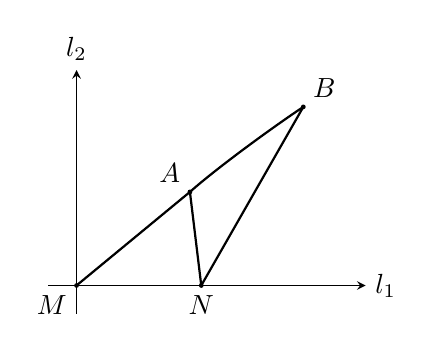
\begin{tikzpicture}[>=stealth, scale=0.72]
  \coordinate (M) at (0,0);
  \coordinate (N) at (2.2,0);
  \coordinate (A) at (2.0,1.65);
  \coordinate (B) at (4.0,3.15);
  \draw[->] (-0.5,0)--(5.1,0) node[right] {$l_1$};
  \draw[->] (0,-0.5)--(0,3.8) node[above] {$l_2$};
  \draw[thick] (A) .. controls (2.45,2.05) and (3.4,2.75) .. (B);
  \draw[thick] (A)--(M) (A)--(N) (B)--(N);
  \draw[dashed] (M)--(A);
  \fill (M) circle (1.2pt) node[below left] {$M$};
  \fill (N) circle (1.2pt) node[below] {$N$};
  \fill (A) circle (1.2pt) node[above left] {$A$};
  \fill (B) circle (1.2pt) node[above right] {$B$};
\end{tikzpicture}
\end{center}
\nopagebreak[4]
\Needspace{4\baselineskip}
\textbf{解析}

\Needspace{5\baselineskip}
取坐标原点为 $MN$ 的中点，$x$ 轴沿 $l_1$，并令

\nopagebreak[4]
\[
M=(-2,0),\qquad N=(2,0).
\]

\Needspace{5\baselineskip}
于是 $l_2$ 的方程为 $x=-2$。设曲线段上任一点为 $(x,y)$。该点到 $l_2$ 的距离等于到 $N$ 的距离，所以在图示的 $l_2$ 右侧有

\nopagebreak[4]
\[
x+2=\sqrt{(x-2)^2+y^2}.
\]

\Needspace{5\baselineskip}
平方化简得

\nopagebreak[4]
\[
y^2=8x.
\]

\Needspace{5\baselineskip}
由 $|AM|=\sqrt{17}$、$|AN|=3$，设 $A=(x_A,y_A)$，则

\nopagebreak[4]
\[
(x_A+2)^2+y_A^2=17,\qquad
(x_A-2)^2+y_A^2=9.
\]

相减得 $x_A=1$，再代入得 $y_A^2=8$。按固定源图示取上支，故 $A=(1,2\sqrt2)$。

三角形 $AMN$ 的三边为 $\sqrt{17},3,4$，满足最大边平方小于另外两边平方和，正好符合锐角条件；这也排除了另一坐标原点选择下的钝角分支。

\Needspace{5\baselineskip}
同理，$|BN|=6$ 且 $B$ 在上支，故

\nopagebreak[4]
\[
x_B+2=6,\qquad x_B=4,\qquad y_B=4\sqrt2.
\]

\Needspace{5\baselineskip}
所以曲线段的方程为

\nopagebreak[4]
\[
y^2=8x,\qquad 1\leqslant x\leqslant4,\quad y>0.
\]

\gkanswer{答案：见解析版}

\end{answer}
\begin{answer}
\gksolhead{22}{}

\textbf{题目}：

如图，为处理含有某种杂质的污水，要制造一底宽为 2 米的无盖长方体沉淀箱，污水从 $A$ 孔流入，经沉淀后从 $B$ 孔流出。设箱体的长度为 $a$ 米，高度为 $b$ 米。已知流出的水中该杂质的质量分数与 $a,b$ 的乘积 $ab$ 成反比。现有制箱材料 60 平方米。问当 $a,b$ 各为多少米时，经沉淀后流出的水中该杂质的质量分数最小。（$A\text{、}B$ 孔的面积忽略不计）
\nopagebreak[4]
\begin{center}% 1998 年全国卷理科第 22 题：无盖长方体沉淀箱示意图
\begin{tikzpicture}[>=stealth, scale=0.78]
  \coordinate (A) at (0,0);
  \coordinate (B) at (4.8,0);
  \coordinate (C) at (5.7,0.75);
  \coordinate (D) at (0.9,0.75);
  \coordinate (A1) at (0,2.45);
  \coordinate (B1) at (4.8,2.45);
  \coordinate (C1) at (5.7,3.2);
  \coordinate (D1) at (0.9,3.2);
  \draw[thick] (A)--(B)--(C)--(C1)--(B1)--(A1);
  \draw[thick] (A1)--(D1)--(C1);
  \draw[dashed] (A)--(D)--(C) (A)--(A1) (D)--(D1);
  \draw[dashed] (B)--(B1);
  \fill (A) circle (1.2pt) node[below left] {$A$};
  \fill (B) circle (1.2pt) node[below right] {$B$};
  \node[below] at (2.4,0) {$a$};
  \node[right] at (5.35,1.6) {$b$};
  \node[below] at (5.25,0.35) {$2$};
  \node[above left] at (0.9,2.7) {无盖};
\end{tikzpicture}
\end{center}
\nopagebreak[4]
\Needspace{4\baselineskip}
\textbf{解析}

\Needspace{5\baselineskip}
无盖箱子的底面面积为 $2a$，两个长侧面的面积总和为 $2ab$，两个端面的面积总和为 $4b$。材料约束为

\nopagebreak[4]
\[
2a+2ab+4b=60,
\qquad
a+ab+2b=30.
\]

\Needspace{5\baselineskip}
质量分数与 $ab$ 成反比，所以需要在该约束下使 $ab$ 最大。由约束解出

\nopagebreak[4]
\[
b=\frac{30-a}{a+2},
\qquad
ab=\frac{a(30-a)}{a+2},
\qquad 0<a<30.
\]

\Needspace{5\baselineskip}
对最后一个函数求导：

\nopagebreak[4]
\[
\left(\frac{a(30-a)}{a+2}\right)'
=\frac{60-4a-a^2}{(a+2)^2}
=\frac{(a+10)(6-a)}{(a+2)^2}.
\]

\Needspace{5\baselineskip}
因此它在 $a=6$ 时取得最大值。代回约束：

\nopagebreak[4]
\[
30=6+6b+2b,
\qquad b=3.
\]

所以当 $a=6$ 米、$b=3$ 米时，质量分数最小。

\gkanswer{答案：$a=6$ 米，$b=3$ 米}

\end{answer}
\begin{answer}
\gksolhead{23}{}

\textbf{题目}：

已知斜三棱柱 $ABC-A_1B_1C_1$ 的侧面 $A_1ACC_1$ 与底面 $ABC$ 垂直，$\angle ABC=90^\circ$，$BC=2$，$AC=2\sqrt3$，且 $AA_1\perp A_1C$，$AA_1=A_1C$。

（1） 求侧棱 $A_1A$ 与底面 $ABC$ 所成角的大小；

（2） 求侧面 $A_1ABB_1$ 与底面 $ABC$ 所成二面角的大小；

（3） 求顶点 $C$ 到侧面 $A_1ABB_1$ 的距离。
\nopagebreak[4]
\begin{center}% 1998 年全国卷理科第 23 题：斜三棱柱 ABC-A_1B_1C_1
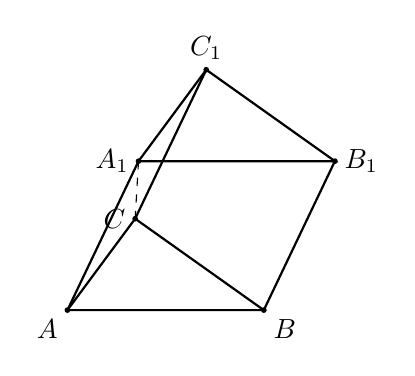
\begin{tikzpicture}[>=stealth, scale=0.86]
  \coordinate (A) at (0,0);
  \coordinate (B) at (2.9,0);
  \coordinate (C) at (1.0,1.35);
  \coordinate (A1) at (1.05,2.2);
  \coordinate (B1) at (3.95,2.2);
  \coordinate (C1) at (2.05,3.55);
  \draw[thick] (A)--(B)--(C)--cycle;
  \draw[thick] (A1)--(B1)--(C1)--cycle;
  \draw[thick] (A)--(A1) (B)--(B1) (C)--(C1);
  \draw[dashed] (A1)--(C) (A)--(C);
  \fill (A) circle (1.2pt) node[below left] {$A$};
  \fill (B) circle (1.2pt) node[below right] {$B$};
  \fill (C) circle (1.2pt) node[left] {$C$};
  \fill (A1) circle (1.2pt) node[left] {$A_1$};
  \fill (B1) circle (1.2pt) node[right] {$B_1$};
  \fill (C1) circle (1.2pt) node[above] {$C_1$};
\end{tikzpicture}
\end{center}
\nopagebreak[4]
\Needspace{4\baselineskip}
\textbf{解析}

\Needspace{5\baselineskip}
在底面取

\nopagebreak[4]
\[
B=(0,0,0),\qquad C=(2,0,0),\qquad A=(0,2\sqrt2,0),
\]

\Needspace{5\baselineskip}
则 $AB=2\sqrt2$、$BC=2$、$AC=2\sqrt3$，满足直角三角形条件。记 $\boldsymbol d=\overrightarrow{AC}=(2,-2\sqrt2,0)$，其长度平方为 $12$。侧面 $A_1ACC_1$ 与底面垂直，故侧棱向量 $\boldsymbol v=\overrightarrow{AA_1}$ 的水平投影沿 $AC$。设

\nopagebreak[4]
\[
\boldsymbol v=\lambda\boldsymbol d+(0,0,h).
\]

\Needspace{5\baselineskip}
由 $AA_1\perp A_1C$ 且 $AA_1=A_1C$，三角形 $AA_1C$ 是等腰直角三角形，故

\nopagebreak[4]
\[
|\boldsymbol v|^2=|\boldsymbol d-\boldsymbol v|^2=\frac{|\boldsymbol d|^2}{2}=6,
\qquad
\boldsymbol v\cdot(\boldsymbol d-\boldsymbol v)=0.
\]

\Needspace{5\baselineskip}
从而 $\boldsymbol v\cdot\boldsymbol d=6$，即 $\lambda=1/2$；再由长度得 $h^2=3$。按图示方向取 $h=\sqrt3$，因此

\nopagebreak[4]
\[
A_1=(1,\sqrt2,\sqrt3),\qquad
B_1=(1,-\sqrt2,\sqrt3).
\]

\gksubpart{(1)}

\Needspace{5\baselineskip}
侧棱向量为

\nopagebreak[4]
\[
\overrightarrow{AA_1}=(1,-\sqrt2,\sqrt3),
\qquad
|\overrightarrow{AA_1}|=\sqrt6.
\]

\Needspace{5\baselineskip}
它与底面所成角记为 $\theta$，则

\nopagebreak[4]
\[
\sin\theta=\frac{\sqrt3}{\sqrt6}=\frac{\sqrt2}{2}.
\]

所以 $\theta=\pi/4$。

\gksubpart{(2)}

\Needspace{5\baselineskip}
平面 $A_1ABB_1$ 经过 $B,A,A_1$，其法向量可取

\nopagebreak[4]
\[
\boldsymbol n=(-\sqrt3,0,1).
\]

\Needspace{5\baselineskip}
底面 $ABC$ 的法向量为 $(0,0,1)$，故两平面所成的锐二面角 $\varphi$ 满足

\nopagebreak[4]
\[
\cos\varphi
=\frac{|(\!-\sqrt3,0,1)\cdot(0,0,1)|}{2}
=\frac12.
\]

所以 $\varphi=\pi/3$。

\gksubpart{(3)}

\Needspace{5\baselineskip}
平面 $A_1ABB_1$ 过原点 $B$，其方程为

\nopagebreak[4]
\[
-\sqrt3x+z=0.
\]

\Needspace{5\baselineskip}
点 $C=(2,0,0)$ 到该平面的距离为

\nopagebreak[4]
\[
\frac{|-\sqrt3\cdot2+0|}{\sqrt{(\sqrt3)^2+1^2}}
=\frac{2\sqrt3}{2}
=\sqrt3.
\]

\gkanswer{答案（1）：$\dfrac\pi4$}

\gkanswer{答案（2）：$\dfrac\pi3$}

\gkanswer{答案（3）：$\sqrt3$}

\end{answer}
\begin{answer}
\gksolhead{24}{}

\textbf{题目}：

设曲线 $C$ 的方程是 $y=x^3-x$，将 $C$ 沿 $x$ 轴、$y$ 轴正向分别平行移动 $t,s$ 个单位长度后得曲线 $C_1$。

（1） 写出曲线 $C_1$ 的方程；

（2） 证明曲线 $C$ 与 $C_1$ 关于点 $A\left(\dfrac t2,\dfrac s2\right)$ 对称；

（3） 如果曲线 $C$ 与 $C_1$ 有且仅有一个公共点，证明 $s=\dfrac{t^3}{4}-t$ 且 $t\neq0$。

\Needspace{4\baselineskip}
\textbf{解析}

\gksubpart{(1)}

\Needspace{5\baselineskip}
曲线沿 $x$ 轴正向平移 $t$、沿 $y$ 轴正向平移 $s$ 后，原坐标中的 $x,y$ 在新曲线上分别对应原曲线的 $x-t,y-s$，故

\nopagebreak[4]
\[
y-s=(x-t)^3-(x-t),
\]

\Needspace{5\baselineskip}
即

\nopagebreak[4]
\[
y=(x-t)^3-x+t+s.
\]

\gksubpart{(2)}

\Needspace{5\baselineskip}
设 $P=(x,y)$ 在 $C$ 上，即 $y=x^3-x$。关于

\nopagebreak[4]
\[
A\left(\frac t2,\frac s2\right)
\]

\Needspace{5\baselineskip}
的对称点为

\nopagebreak[4]
\[
P'=(t-x,s-y).
\]

\Needspace{5\baselineskip}
将其代入 $C_1$ 的左式：

\nopagebreak[4]
\[
(s-y)-s=(t-x-t)^3-(t-x)+t
=-x^3+x.
\]

由于 $y=x^3-x$，右边等于 $-y$，所以 $P'$ 满足 $y'-s=(x'-t)^3-(x'-t)$，即 $P'\in C_1$。反向同理，因此两曲线关于点 $A$ 对称。

\gksubpart{(3)}

\Needspace{5\baselineskip}
公共点的横坐标满足

\nopagebreak[4]
\[
x^3-x=(x-t)^3-x+t+s,
\]

\Needspace{5\baselineskip}
即

\nopagebreak[4]
\[
3tx^2-3t^2x+t^3-t-s=0.
\]

\Needspace{5\baselineskip}
若 $t=0$，两曲线或者重合或者没有交点，不可能恰有一个公共点，所以 $t\neq0$。当 $t\neq0$ 时，恰有一个公共点要求上述关于 $x$ 的二次方程判别式为零：

\nopagebreak[4]
\[
\begin{aligned}
\Delta
&=(-3t^2)^2-4(3t)(t^3-t-s)\\
&=-3t(t^3-4t-4s)=0.
\end{aligned}
\]

\Needspace{5\baselineskip}
因此

\nopagebreak[4]
\[
s=\frac{t^3}{4}-t,\qquad t\neq0.
\]

\gkanswer{答案（1）：$y=(x-t)^3-x+t+s$}

\gkanswer{答案（2）：见解析版}

\gkanswer{答案（3）：见解析版}

\end{answer}
\begin{answer}
\gksolhead{25}{}

\textbf{题目}：

已知数列 $\{b_n\}$ 是等差数列，$b_1=1$，$b_1+b_2+\cdots+b_{10}=145$。

（1） 求数列 $\{b_n\}$ 的通项 $b_n$；

\Needspace{5\baselineskip}
（2） 设数列 $\{a_n\}$ 的通项

\nopagebreak[4]
\[
a_n=\log_a\left(1+\frac1{b_n}\right)
\]

（其中 $a>0$，且 $a\neq1$），记 $S_n$ 是数列 $\{a_n\}$ 的前 $n$ 项和。试比较 $S_n$ 与 $\dfrac13\log_a b_{n+1}$ 的大小，并证明你的结论。

\Needspace{4\baselineskip}
\textbf{解析}

\gksubpart{(1)}

\Needspace{5\baselineskip}
设等差数列公差为 $d$。由

\nopagebreak[4]
\[
\frac{10(b_1+b_{10})}{2}=145,\qquad b_1=1,
\]

\Needspace{5\baselineskip}
得 $b_{10}=28$，从而

\nopagebreak[4]
\[
d=\frac{28-1}{9}=3.
\]

\Needspace{5\baselineskip}
所以

\nopagebreak[4]
\[
b_n=1+(n-1)3=3n-2.
\]

\gksubpart{(2)}

\Needspace{5\baselineskip}
由上式

\nopagebreak[4]
\[
a_n=\log_a\left(1+\frac1{3n-2}\right)
=\log_a\frac{3n-1}{3n-2}.
\]

\Needspace{5\baselineskip}
对每个 $n\geqslant1$，令 $u_n=1/(3n-2)>0$。则

\nopagebreak[4]
\[
(1+u_n)^3>1+3u_n
=\frac{3n+1}{3n-2}.
\]

\Needspace{5\baselineskip}
将 $n=1,\ldots,N$ 的不等式相乘，得到

\nopagebreak[4]
\[
\prod_{n=1}^{N}
\left(\frac{3n-1}{3n-2}\right)^3
>
\prod_{n=1}^{N}\frac{3n+1}{3n-2}
=\frac41\cdot\frac74\cdots\frac{3N+1}{3N-2}
=3N+1=b_{N+1}.
\]

\Needspace{5\baselineskip}
所以当 $a>1$ 时，$\log_a$ 保持不等号方向：

\nopagebreak[4]
\[
3S_N>\log_a b_{N+1},
\qquad
S_N>\frac13\log_a b_{N+1}.
\]

\Needspace{5\baselineskip}
当 $0<a<1$ 时，$\log_a$ 为减函数，不等号方向反向：

\nopagebreak[4]
\[
S_N<\frac13\log_a b_{N+1}.
\]

\gkanswer{答案（1）：$b_n=3n-2$}

\gkanswer{答案（2）：若 $a>1$，则 $S_n>\dfrac13\log_a b_{n+1}$；若 $0<a<1$，则 $S_n<\dfrac13\log_a b_{n+1}$。}

\end{answer}